\chapter{Design and Implementation of the Reward System}
\minitoc
\newpage

\setcounter{secnumdepth}{0} % Set the section counter to 0 so next section is not counted in toc
% ----------------------- Introduction ----------------------- %
\section{Introduction}

In this chapter, we unveil the inaugural release of the reward system, a strategic enhancement by Aermax Company aimed at motivating subcontractors (workers). Integral to the Aermax project, this system reflects our comprehensive design considerations, agile planning, and meticulous implementation efforts. Through this initiative, we underscore our commitment to fostering a motivated and engaged workforce.

\section{Sprints Backlog}
During the Sprint Planning meeting, the effort for each task in the first and second sprint backlogs was assessed based on the total working hours required. The prioritization of these backlog items is depicted through their sequence in the table, with items placed at the top representing higher urgency. Additionally, the accompanying image showcases the board that serves as our operational platform at Incedo.

 \begin{figure}[H]
    \centering
    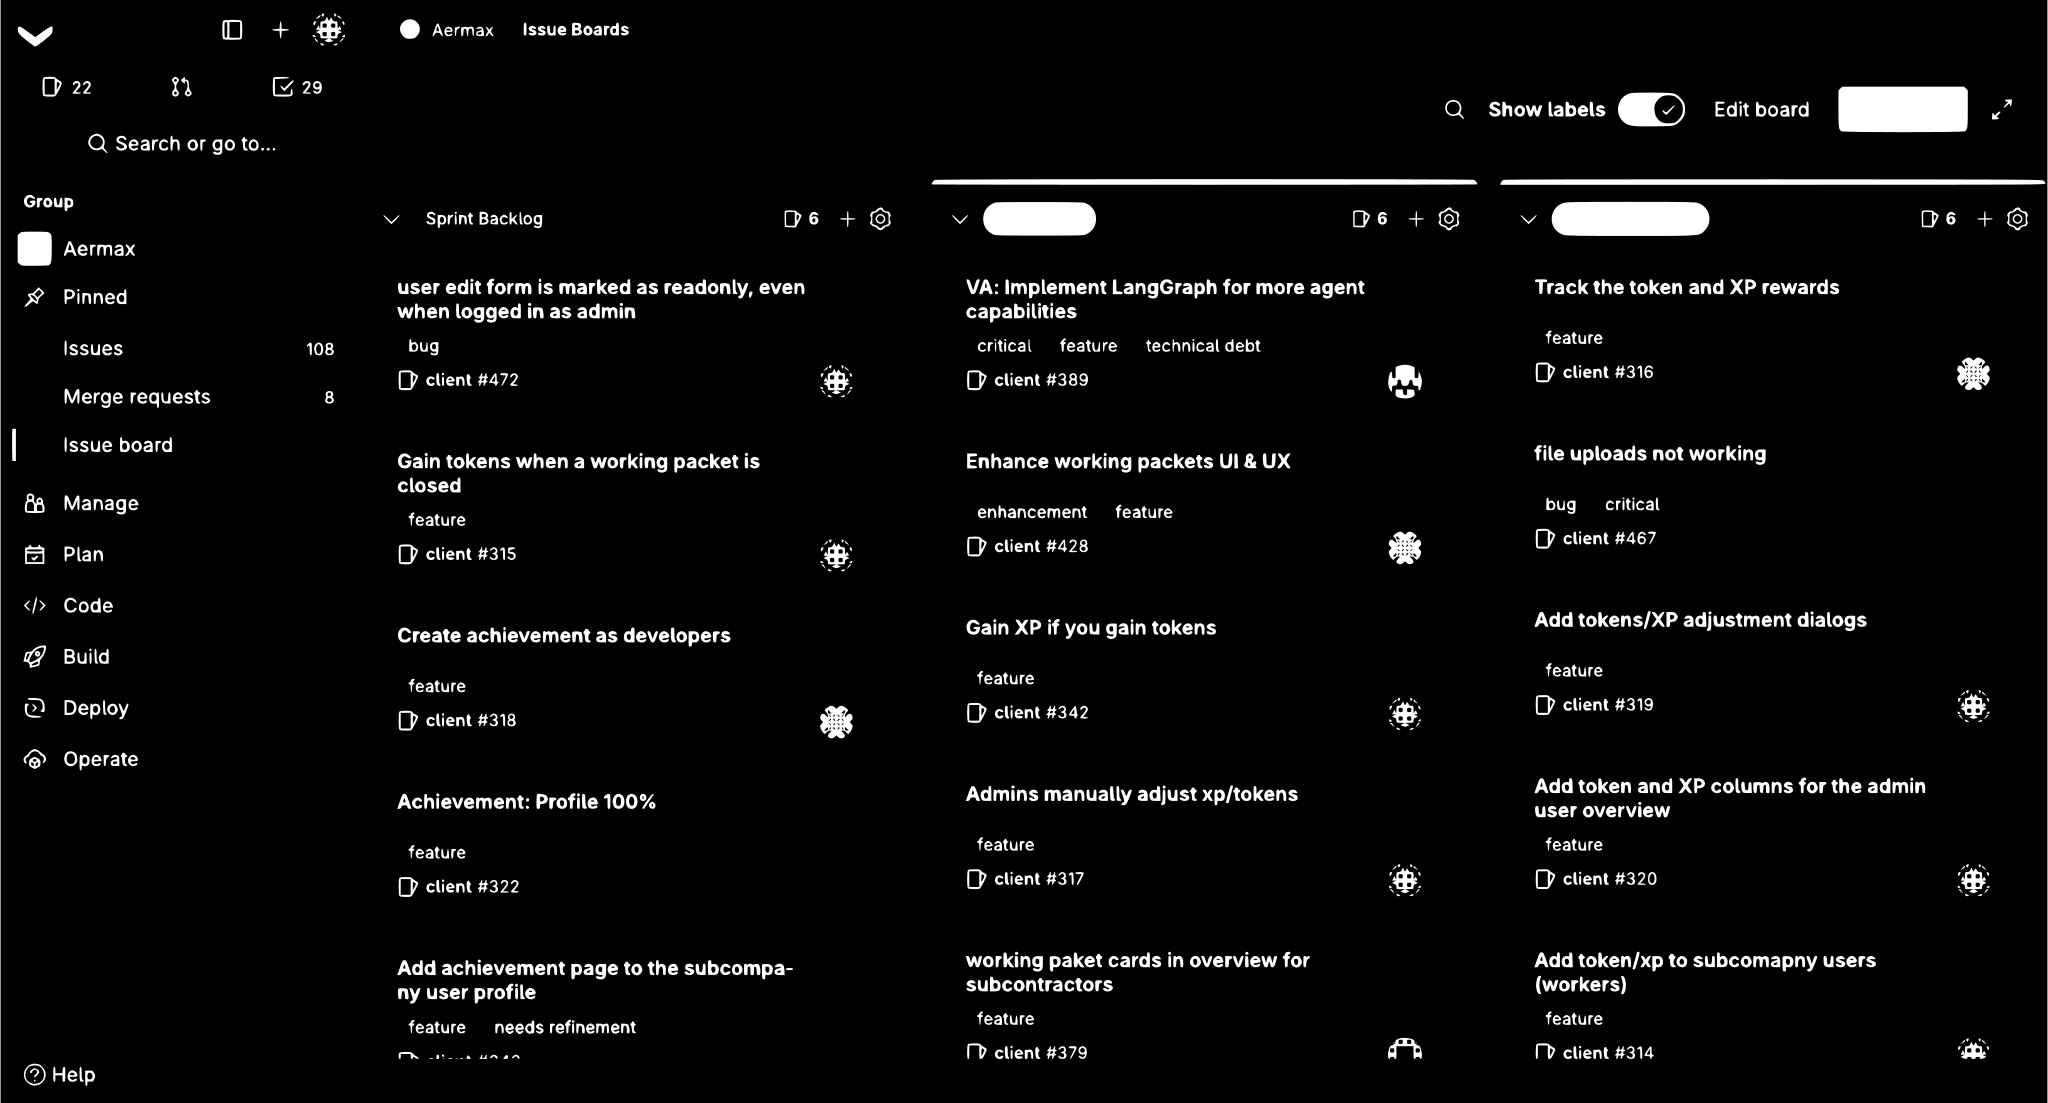
\includegraphics[width=0.9\textwidth]{src/assets/chapters/reward-system-backloog.png}
    \caption{Aermax Project Sprint Backlog and Issue Board Snapshot}
    \label{fig:sprint_backlog_and_issue_board}
\end{figure}

\begin{table}[H]
\centering
\caption{Backlog of Sprint 2}
\label{tab:backlog_sprint_2}
\begin{tabular}{|c|p{4cm}|p{6cm}|c|}
\hline
\textbf{Sprint} & \textbf{Epic} & \textbf{User Story} & \textbf{Estimation (hours)} \\ \hline
2 & Secure Reward System Integration with Keycloak Authentication & Reward Access Security & 9 \\ \hline
2 & Token and XP Management & Add tokens/XP adjustment dialogs & 8 \\ \hline
2 & Token and XP Management & Add token and XP columns for the admin user overview & 10 \\ \hline
2 & Token and XP Management & Add token/xp to subcompany users (workers) & 2 \\ \hline
2 & Token and XP Management & Admins manually adjust xp/tokens & 4 \\ \hline
2 & Token and XP Management & Gain XP if you gain tokens & 5 \\ \hline
2 & Achievements and Rewards Management & Create achievement as developers & 6 \\ \hline
2 & Achievements and Rewards Management & Achievement: Profile 100\% & 6 \\ \hline
2 & Achievements and Rewards Management & Add achievement page to the subcompany user profile & 5 \\ \hline
2 & Achievements and Rewards Management & Add checkbox in user overview to ban a user from gaining tokens & 3 \\ \hline
2 & Achievements and Rewards Management & Gain tokens when a working packet is closed & 13 \\ \hline
\end{tabular}
\end{table}


\section{Specification}

In this section, a detailed breakdown of selected user stories is presented in a structured table layout to facilitate clear documentation and reference. Each user story is accompanied by four essential components:
\begin{itemize}
    \item \textbf{Preconditions:} Outlines the necessary conditions or prerequisites required prior to the initiation of the user story.
    \item \textbf{Business Rules:} Defines the critical constraints, policies, and conditions that dictate the software's operation in response to user inputs.
    \item \textbf{Technical Specifications:} Details the technical requirements, technologies, and architectural considerations essential for actualizing the user story.
    \item \textbf{Acceptance Criteria:} Lists the specific conditions that must be fulfilled for the user story to be regarded as complete and ready for integration.
\end{itemize}

\begin{longtable}{|m{3cm}|m{12cm}|}
\caption{User Stories Specification} \label{tab:user_stories_specification} \\
\hline
\textbf{Epic} & \textbf{User Story} \\
\hline
\endfirsthead
\multicolumn{2}{c}{{\tablename\ \thetable{} -- continued from previous page}} \\
\hline
\textbf{Epic} & \textbf{User Story} \\
\hline
\endhead
\hline
\multicolumn{2}{r}{{Continued on next page}} \\
\endfoot
\hline
\endlastfoot

Secure Reward System Integration with Keycloak Authentication &
\textbf{Preconditions:} \newline A reward system is already in place but lacks secure user authentication. Keycloak is chosen as the authentication solution, ready for setup. \newline
\textbf{Business Rules:} \newline Access to the reward system is strictly limited to verified users. Users must log in through Keycloak, ensuring their identity is securely confirmed. Each user's access rights are determined based on their role. \newline
\textbf{Technical Specifications:} \newline Implement a secure login system using Keycloak. Customize login settings to fit our specific needs, including how users are verified and the level of access they have. Use special security checks to continuously verify that user interactions are safe and authorized. \newline
\textbf{Acceptance Criteria:} \newline Users cannot access the reward system without logging in through Keycloak. After logging in, the system identifies the user's role and grants access accordingly. The reward system logs and monitors each user's actions. The integration passes all security tests. \\
\hline

Token and XP Management &
\textbf{Preconditions:} \newline A functional admin dashboard exists. Users and subcompany (worker) accounts are distinguishable within the system. \newline
\textbf{Business Rules:} \newline Only authorized administrators can view and adjust tokens and XP. Token and XP adjustments must be logged for transparency and auditing. The relationship between token acquisition and XP gains is predefined. \newline
\textbf{Technical Specifications:} \newline Enhance the admin dashboard with features to add and adjust tokens/XP through user-friendly dialogs. Update the admin user overview to include token and XP columns. Allow tokens and XP to be allocated to subcompany users. Enable admins to manually adjust tokens and XP. \newline
\textbf{Acceptance Criteria:} \newline Admins can manage tokens and XP effectively. Adjustments to tokens and XP are accurately logged. Subcompany users receive tokens and XP as allocated by admins. The automatic XP gain feature activates upon token acquisition. \\
\hline

Achievements and Rewards Management &
\textbf{Preconditions:} \newline A system for tracking user activities and achievements is in place. Subcompany and user profiles are established within the system. \newline
\textbf{Business Rules:} \newline Developers can create and define achievements. Achievements must be visible and accessible to users. Administrators can restrict users from earning tokens. Token rewards are aligned with specific user actions. \newline
\textbf{Technical Specifications:} \newline Implement functionality for developers to create achievements. Develop an achievements page accessible from the subcompany user profile. Introduce user restrictions for token earning. Establish a mechanism that awards tokens to users upon completing tasks. \newline
\textbf{Acceptance Criteria:} \newline Developers can create new achievements without issues. Achievements are properly tracked and awarded. Administrators can apply restrictions to users' ability to earn tokens. Users receive tokens upon completing work packets. \\
\hline

\end{longtable}

\section{Initial Planning and Conceptualization Phase}

\subsection{Overview}
This phase initiates the development of a reward system, aimed at closely aligning with customer needs through a structured approach. It sets the groundwork for translating these needs into a functional design, ensuring the system not only meets but anticipates user requirements. Our focus here is on establishing a clear vision and framework that will guide the entire development process, from conceptualization to implementation, fostering a user-centric and impactful solution.

\subsection*{System Goals and Objectives}
The primary goal of the reward system is to enhance user engagement and motivation within our software ecosystem. Specifically, the system aims to:
\begin{itemize}
    \item \textbf{Increase User Engagement:} Encourage active participation and interaction with the software by providing incentives and rewards for desired behaviours.
    \item \textbf{Drive User Motivation:} Motivate users to achieve specific goals, complete tasks, and contribute positively to the community through a structured rewards program.
    \item \textbf{Enhance User Experience:} Improve overall satisfaction and enjoyment of the software by offering tangible rewards, recognition, and opportunities for progression.
    \item \textbf{Foster Community Growth:} Facilitate the growth and development of a vibrant user community by fostering collaboration, competition, and a sense of belonging through the reward system.
\end{itemize}
These objectives align with our overarching mission to create a dynamic and engaging software platform that not only meets but exceeds user expectations, ultimately leading to increased user retention and loyalty.

\subsection{High-Level System Overview}
This section offers a conceptual snapshot of our reward system, outlining its key components and their anticipated interactions. Below, we delve into the global use cases, illustrating the system's functionality in greater detail.
 \begin{figure}[H]
    \centering
    \includegraphics[width=1\textwidth]{src/assets/chapters/raward-sysetm-usecase.drawio.png}
    \caption{Aermax Global Use Case Diagram}
    \label{fig:globa_usecase_diagram}
\end{figure}

\subsection{Initial System Architecture Sketch}
In this section, we present the Initial System Architecture Sketch, which offers a visual representation of the foundational structure of our reward system. This diagram serves as a high-level blueprint, illustrating the primary components and their interactions within the system. It is designed to clarify the modular approach we have adopted, ensuring scalability, maintainability, and robustness.

The architecture is segmented into distinct modules, each responsible for a core aspect of the system's functionality:
\begin{itemize}
    \item \textbf{Token and XP Ledger:} Manages the currency of motivation - tokens and experience points.
    \item \textbf{Achievements Management:} Tracks and administers user accomplishments.
    \item \textbf{User Authentication:} Secures the system, ensuring that users can safely access their data and functionalities.
\end{itemize}

As we progress through the stages of development, this sketch may evolve to incorporate feedback and additional features, ultimately guiding us towards a fully-realized implementation that aligns with our vision of a dynamic and engaging user experience.

 \begin{figure}[H]
    \centering
    \includegraphics[width=1\textwidth]{src/assets/chapters/reward-deployement-diagram.drawio.png}
    \caption{ Reward System Architecture Overview}
    \label{fig:reward_system_architecture_overview}
\end{figure}

\section{Design}
This phase of the project builds upon our foundational work to refine and expand the architecture of our reward system. We delve into key considerations, decisions, and enhancements introduced in this release, focusing particularly on how our models support the reward functionalities.

\subsection{Static Modeling}
The static modeling phase has been pivotal in defining the core structure of our reward system. We have continued to refine our data models and database schema to align with our evolving functional requirements and business rules.

\subsubsection{Domain Model}
We have structured our reward system around three primary classes: RewardLog, UserRewards, and Achievement. These classes are designed to seamlessly interact within our system to facilitate efficient reward management and user engagement through achievements.

\subsection{Classes Description}
\begin{tabular}{|l|p{10cm}|}
\hline
\textbf{Class Name} & \textbf{Description} \\
\hline
RewardLog & Models individual reward transactions, capturing details like user ID, reward type (XP, token), and the source of the reward (e.g., completing a task or manual adjustment). \\
\hline
UserRewards & Models the cumulative rewards and achievements for a user, providing a comprehensive overview of their progress and tokens. \\
\hline
Achievement & Details the achievements that users can earn, including the criteria for earning them and the rewards associated with them. \\
\hline
\end{tabular}

For these classes, we have defined the following associations:
\begin{itemize}
    \item Each UserRewards document embeds an array of Achievement subdocuments, reflecting the user's progress towards various achievements.
    \item RewardLog entries are linked to specific actions or events, such as achievement completions, which can update the UserRewards document.
\end{itemize}
 we illustrate the extension of our class diagram, highlighting newly added classes and associations for clarity.

\subsubsection{Data Dictionary}
In table IV.4, we provide a comprehensive overview of the key data elements used in our model, detailing how they interact and are structured within our database. This dictionary will cover the essential attributes for each class, such as userId, type, and source in RewardLog, and how they are indexed for performance and uniqueness.

\subsubsection{Logical Data Model}
Building on the foundation laid by the first version of our logical data model, our MVP, we now present an updated model that retains the original structure while introducing necessary expansions for this release. This updated model provides insights into the relationships and structure of our data entities, reflecting the full scope of the initial solution. Figure IV.2 illustrates the class diagram, showing how new and existing entities are interconnected within our system.


 \begin{figure}[H]
    \centering
    \includegraphics[width=0.9\textwidth]{src/assets/chapters/reward--system-classDiagram.drawio.png}
    \caption{ Data Model Architecture}
    \label{fig:reward_system_architecture_overview}
\end{figure}
\subsection{Data Dictionary}

\subsection{Data Dictionary for RewardLog}
\begin{tabular}{|l|p{9cm}|l|l|}
\hline
\textbf{Field} & \textbf{Description} & \textbf{Type} & \textbf{Constraints} \\
\hline
userId & User's unique identifier & string & Required \\
\hline
type & Type of reward (e.g., xp, token) & enum & Required \\
\hline
amount & Amount of reward given & number & Required \\
\hline
source & Source of reward (e.g., close\_packet, manual\_adjustment, achievement) & enum & Required \\
\hline
packetId & Identifier for the reward packet, if applicable & string & Optional \\
\hline
adminId & Administrator's identifier managing the reward & string & Optional \\
\hline
achievementId & Reference to associated achievement & ObjectId & Optional \\
\hline
\end{tabular}

\subsection{Data Dictionary for UserRewards}
\begin{tabular}{|l|l|l|l|}
\hline
\textbf{Field} & \textbf{Description} & \textbf{Type} & \textbf{Constraints} \\
\hline
userId & User's unique identifier & string & Required \\
\hline
xp & Total experience points & number & Default: 0 \\
\hline
tokens & Total tokens & number & Default: 0 \\
\hline
reason & Reason for reward adjustment & string & Optional \\
\hline
achievements & Array of achievements (subdocument) & subdocument & Optional \\
\hline
isBanned & Whether the user is banned from receiving rewards & boolean & Default: false \\
\hline
\end{tabular}

\subsection{Data Dictionary for Achievement}
\begin{tabular}{|l|l|l|l|}
\hline
\textbf{Field} & \textbf{Description} & \textbf{Type} & \textbf{Constraints} \\
\hline
name & Name of the achievement & string & Required, Unique \\
\hline
reward & Reward amount for achieving this milestone & number & Default: 0 \\
\hline
step & Incremental steps required to achieve the milestone & number & Default: 1 \\
\hline
maximum & Maximum progress needed to complete the achievement & number & Default: 1 \\
\hline
title & Title of the achievement & string & Required \\
\hline
description & Description of the achievement & string & Required \\
\hline
imageUrl & URL of the image associated with the achievement & string & Required \\
\hline
createdBy & Identifier of the user who created the achievement & string & Required \\
\hline
updatedBy & Identifier of the user who last updated the achievement & string & Required \\
\hline
\end{tabular}

\section{Dynamic Modeling}
In this section, we explore the dynamic aspects of our reward system, focusing on the interactions and communication behaviors between components and actors within our system. 

\subsection{User Interaction Workflow}
This flowchart illustrates the dynamic interactions users have with our system, depicting the process flow and decision points encountered during typical user sessions. Understanding these interactions helps us optimize the user experience and streamline how rewards and achievements are managed in response to user actions.

 \begin{figure}[H]
    \centering
    \includegraphics[width=0.9\textwidth]{src/assets/chapters/Reward-System_Activity-Flow.png}
    \caption{ Data Model Architecture}
    \label{fig:reward_system_architecture_overview}
\end{figure}

\subsection{Admin Sequence Diagram}
The admin sequence diagram concisely outlines the steps an admin takes to manage the reward system, from login through various tasks like adjusting tokens and XP. It clarifies the admin's interactions within the system and assists in streamlining administrative functions for optimal efficiency.


% Here you would include your admin sequence diagram figure
\begin{figure}[H]
    \centering
    \includegraphics[width=0.9\textwidth]{src/assets/chapters/AdminSequencediagram.png}
    \caption{Admin Sequence Diagram for the Reward System}
    \label{fig:admin_sequence_diagram}
\end{figure}
\subsection{Subcompany User Sequence Diagram}
This sequence diagram depicts the key steps a subcompany user takes within the reward system, from login to earning rewards. It streamlines the user journey, highlighting how users interact with the system and the resulting workflow, thereby ensuring an experience that is both user-friendly and aligned with the system's goals.


% Include the figure for the subcompany user sequence diagram here
\begin{figure}[H]
    \centering
    \includegraphics[width=0.9\textwidth]{src/assets/chapters/subbcomapny_user_sequence_diagram.png}
    \caption{Sequence Diagram for Subcompany User Interactions in the Reward System}
    \label{fig:subcompany_user_sequence_diagram}
\end{figure}

\section{Software Architecture}
Following the design phase, we chose to implement a separate microservice built with NestJS to enhance the scalability and maintainability of our reward system. This microservice architecture allows for isolated development and deployment, which simplifies updates and scaling operations.

\subsection{Microservice Architecture}
The new microservice integrates seamlessly with existing services such as the operation-service and user-service. It communicates via RabbitMQ, a robust message broker that ensures reliable and efficient message handling between services. This approach not only improves the system's responsiveness but also its overall resilience, allowing each component to operate independently yet cohesively.

\paragraph{Benefits of NestJS and RabbitMQ:}
\begin{itemize}
    \item \textbf{NestJS:} Provides a scalable framework for building efficient and fail-safe systems, thanks to its use of modern JavaScript features and its integration with TypeScript.
    \item \textbf{RabbitMQ:} Facilitates secure and flexible cross-service communication, enhances fault tolerance, and manages load effectively, even under high demand.
\end{itemize}

This architectural decision supports our goal of creating a dynamic, reliable, and scalable reward system, prepared to handle increasing loads and complexity as the Aermax platform grows.

\begin{figure}[H]
    \centering
    \includegraphics[width=0.9\textwidth]{src/assets/chapters/rmq.png}
    \caption{Microservice Communication Example via RabbitMQ in the Reward System}
    \label{fig:microservice_communication_rabbitmq}
\end{figure}

\section{Technology Stack and Framework Selection}

\subsection*{Why We Chose RabbitMQ}
The decision to choose RabbitMQ as our message broker was based on specific needs for our system's communication and architecture:

\begin{itemize}
    \item \textbf{Decoupling of Services:} RabbitMQ provides independence between services, facilitating a more maintainable and flexible architecture.
    \item \textbf{Asynchronous Communication:} It enables services to communicate without synchronous waits, increasing efficiency.
    \item \textbf{Scalability:} RabbitMQ supports even message distribution, which is essential for scaling services effectively.
    \item \textbf{Reliability and Fault Tolerance:} It ensures message delivery reliability, even when some services are down.
    \item \textbf{Centralized Management:} RabbitMQ offers centralized management of message flows, improving monitoring and control.
    \item \textbf{Ordering and Prioritization:} It manages the order and priority of message handling, which is crucial for process sequencing.
\end{itemize}

\paragraph*{Comparison of Message Brokers}
Below is a comparison of message brokers supported by NestJS, highlighting their main features and common use cases:

\begin{table}[H]
\centering
\caption{Comparison of Message Brokers}
\label{tab:message_brokers_comparison}
\begin{tabular}{|l|p{6cm}|p{5cm}|}
\hline
\textbf{Message Broker} & \textbf{Main Features} & \textbf{Use Case} \\
\hline
Kafka & High throughput, scalability, fault tolerance, and durable storage & Event streaming, log aggregation \\
\hline
MQTT & Lightweight, low bandwidth requirement, designed for IoT devices & IoT, real-time messaging \\
\hline
RabbitMQ & Flexible routing, reliable messaging, multiple protocol support & Complex routing, service decoupling \\
\hline
Redis & In-memory data structure, high performance, supports pub/sub & Caching, real-time analytics \\
\hline
NATS & At-most-once delivery, lightweight, supports queuing & Microservices communication, IoT \\
\hline
gRPC & High-performance RPC, supports bi-directional streaming & Inter-service communication, APIs \\
\hline
\end{tabular}
\end{table}

Our selection of RabbitMQ aligns with our system's need for a robust, reliable, and flexible communication backbone.

\section{Message Broker Operation}

\subsection*{How Does a Message Broker Work?}
A message broker like RabbitMQ plays a critical role in modern software architectures by managing communications between different parts of a system. It acts as a middleman that allows services to send and receive messages without knowing the complexities of each other’s design, location, or technology.

\paragraph*{Example: PDF Creation Process}
Consider a PDF creation process in a web application, which is a typical use case for a message broker. Here’s how it operates:

\begin{enumerate}
    \item A user initiates a PDF creation request from the website application interface.
    \item The application, acting as the \textbf{Producer}, publishes a message to the RabbitMQ \textbf{Exchange}. This message contains the user’s information and the request details.
    \item RabbitMQ routes the message to the appropriate \textbf{Queue} based on the message's content and the queue's binding rules.
    \item The \textbf{Consumer}, which could be a PDF Creator Worker, listens to the queue, consumes the message, and processes the PDF creation.
\end{enumerate}

This process showcases how RabbitMQ facilitates asynchronous communication, ensuring the application’s responsiveness and reliability. The Producer is decoupled from the Consumer, allowing for independent scaling and maintenance.

\begin{figure}[H]
    \centering
    \includegraphics[width=0.9\textwidth]{src/assets/chapters/rabbitmqexample.png} % Replace with your image path
    \caption{Example of Message Broker Workflow in PDF Creation}
    \label{fig:message_broker_workflow}
\end{figure}

The diagram (Figure \ref{fig:message_broker_workflow}) visualizes this workflow, clarifying the roles of Producers, Exchanges, Queues, and Consumers within the RabbitMQ ecosystem.

\section{NestJS as the Development Framework}

NestJS was selected for its:

\begin{itemize}
    \item Strong support for TypeScript, enhancing code reliability.
    \item Modular architecture, which simplifies scalability and maintenance.
    \item Built-in support for microservices and integration with RabbitMQ.
    \item Dependency injection system, promoting code modularity and reusability.
    \item Growing community and rich ecosystem, providing extensive resources.
    \item Similarity to Angular, offering an easier learning curve for developers.
\end{itemize}

These attributes of NestJS align well with our system’s goals for robust and maintainable microservice development.

